\documentclass[extrafontsizes,60pt,twocolumn]{memoir}
\setstocksize{48in}{96in}
\settrimmedsize{48in}{96in}{*}
\setlrmarginsandblock{1in}{1in}{*}
\setulmarginsandblock{1.4in}{20mm}{*}

\usepackage[svgnames]{xcolor}
\usepackage[none]{hyphenat}
\usepackage{graphicx}
\usepackage{booktabs}
\usepackage[font=small,labelfont=bf]{caption}
\usepackage{amsfonts, amsmath, amsthm, amssymb}
\usepackage{wrapfig}
\usepackage{lipsum,adjustbox}
\usepackage[absolute,overlay]{textpos}
\usepackage{multirow}
\usepackage{titlesec}
\usepackage{cuted}
\usepackage[inline]{enumitem}
\usepackage{url}
\usepackage{tikz,pgfplots,pgfplotstable}
\usepackage{tikz-dependency}
\usepackage[most]{tcolorbox}
\usepackage[charter]{mathdesign}
\usetikzlibrary{arrows.meta}
\captionsetup{labelformat=empty}
\graphicspath{{figures/}}

\begin{document}

\begin{strip}
  \begin{center}
    \HUGE\color{NavyBlue}
    \textbf{Content Differences in Syntactic and Semantic Representations}
  \end{center}
  \hfill
  \begin{minipage}[b]{0.4\linewidth}
    {\large \textbf{Daniel Hershcovich}\textsuperscript{1,2} \&
	   \textbf{Omri Abend}\textsuperscript{2} \&
	   \textbf{Ari Rappoport}\textsuperscript{2} \\[0.5cm]}
    $^1$The Edmond and Lily Safra Center for Brain Sciences \\
      $^2$School of Computer Science and Engineering \\
      \setlength{\columnseprule}{0pt}
      The Hebrew University of Jerusalem \\
      \texttt{\{danielh,oabend,arir\}@cs.huji.ac.il}
  \end{minipage}
  \begin{minipage}[b]{.06\linewidth}
    
\includegraphics[width=\linewidth]{elsc_logo.png}
  \end{minipage}
  \begin{minipage}[b]{.13\linewidth}
    
\includegraphics[width=\linewidth]{huji_banner.png}
    
\includegraphics[width=1.04\linewidth]{cse_banner.jpg}
  \end{minipage}
  \begin{minipage}[b]{.04\linewidth}
    
\includegraphics[width=\linewidth]{huji_logo.jpg}
  \end{minipage}
  \hfill
  \vspace{2cm}
  \titlespacing*{\section}{0pt}{8mm}{5mm}
  \begin{adjustbox}{margin=5mm,frame,minipage=.73\linewidth,center}
    \Large\color{Navy}\centering
    Corpus and analysis of shared annotations with
    \textbf{\color{blue} Universal Conceptual Cognitive Annotation (UCCA)} and
    \textbf{\color{red} Universal Dependencies (UD)}. \\
  \end{adjustbox}
  \begin{center}
    \Large\texttt{bit.ly/{\color{blue}ucca}{\color{red}ud}}
  \end{center}
\end{strip}

%----------------------------------------------------------------------------------------


\color{Black}
\tcbset{
    colback=gray!40,
    width=\columnwidth,
    colframe=white
    }
    
\begin{tcolorbox}
\end{tcolorbox}

\vfill

\section*{Unified DAG Format}

We convert UD into a UCCA-like format supported by TUPA, by inserting non-terminal nodes.

\begin{minipage}{.42\columnwidth}
  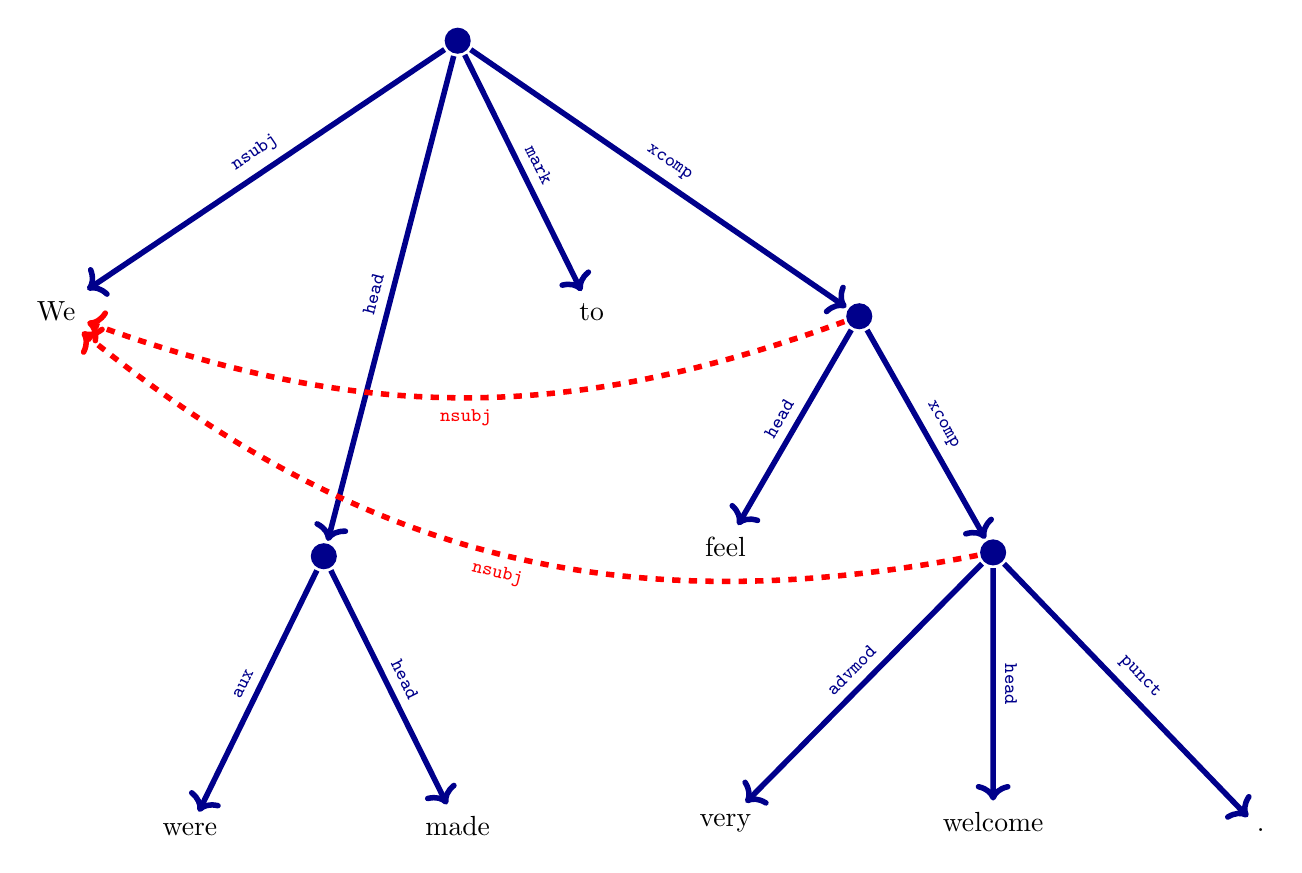
\begin{tikzpicture}[-{Latex[length=5mm]}, color=DarkBlue, line width=2pt,
      every node/.append style={sloped,anchor=south,auto=false,font=\scriptsize\ttfamily},
      sibling distance=34mm, ->,
        every circle node/.append style={fill=DarkBlue},
        level 1/.style={level distance=37mm},
        level 2/.style={level distance=32mm},
        level 3/.style={level distance=37mm}]
      \tikzstyle{word} = [font=\rmfamily,color=black]
      \node (ROOT) [circle] {}
        child {node (We) [word] {We} edge from parent node[midway,above,sloped] {\scriptsize nsubj}}
        child {node {}
        {
	        child {node (weremade) [circle] {}
	        {
	          child {node [word] {were} edge from parent node[midway,above,sloped] {\scriptsize aux}}
	          child {node [word] {made} edge from parent node[midway,above,sloped] {\scriptsize head}}
	        } edge from parent [draw=none]}
        } edge from parent [draw=none]}
        child {node [word] {to} edge from parent node[midway,above,sloped] {\scriptsize mark}}
        child {node (feelverywelcome) [circle] {}
        {
          child {node [word] {feel} edge from parent node[midway,above,sloped] {\scriptsize head}}
          child {node (verywelcome) [circle] {}
          {
            child {node [word] {very} edge from parent node[midway,above,sloped] {\scriptsize advmod}}
            child {node [word] {welcome} edge from parent node[midway,above,sloped] {\scriptsize head}}
            child {node [word] {.} edge from parent node[midway,above,sloped] {\scriptsize punct}}
          } edge from parent node[midway,above,sloped] {\scriptsize xcomp} }
        } edge from parent node[midway,above,sloped] {\scriptsize xcomp} }
      ;
      \draw[->] (ROOT) to node [midway,above,sloped] {\scriptsize head} (weremade);
      \draw[dashed,red,->,bend left=25] (verywelcome) to node [midway,below,sloped] {\scriptsize nsubj} (We);
      \draw[dashed,red,->,bend left=20] (feelverywelcome) to node [midway,below,sloped] {\scriptsize nsubj} (We);
  \end{tikzpicture}
\end{minipage}
\begin{minipage}{.48\columnwidth}
    \scalebox{.8}{
	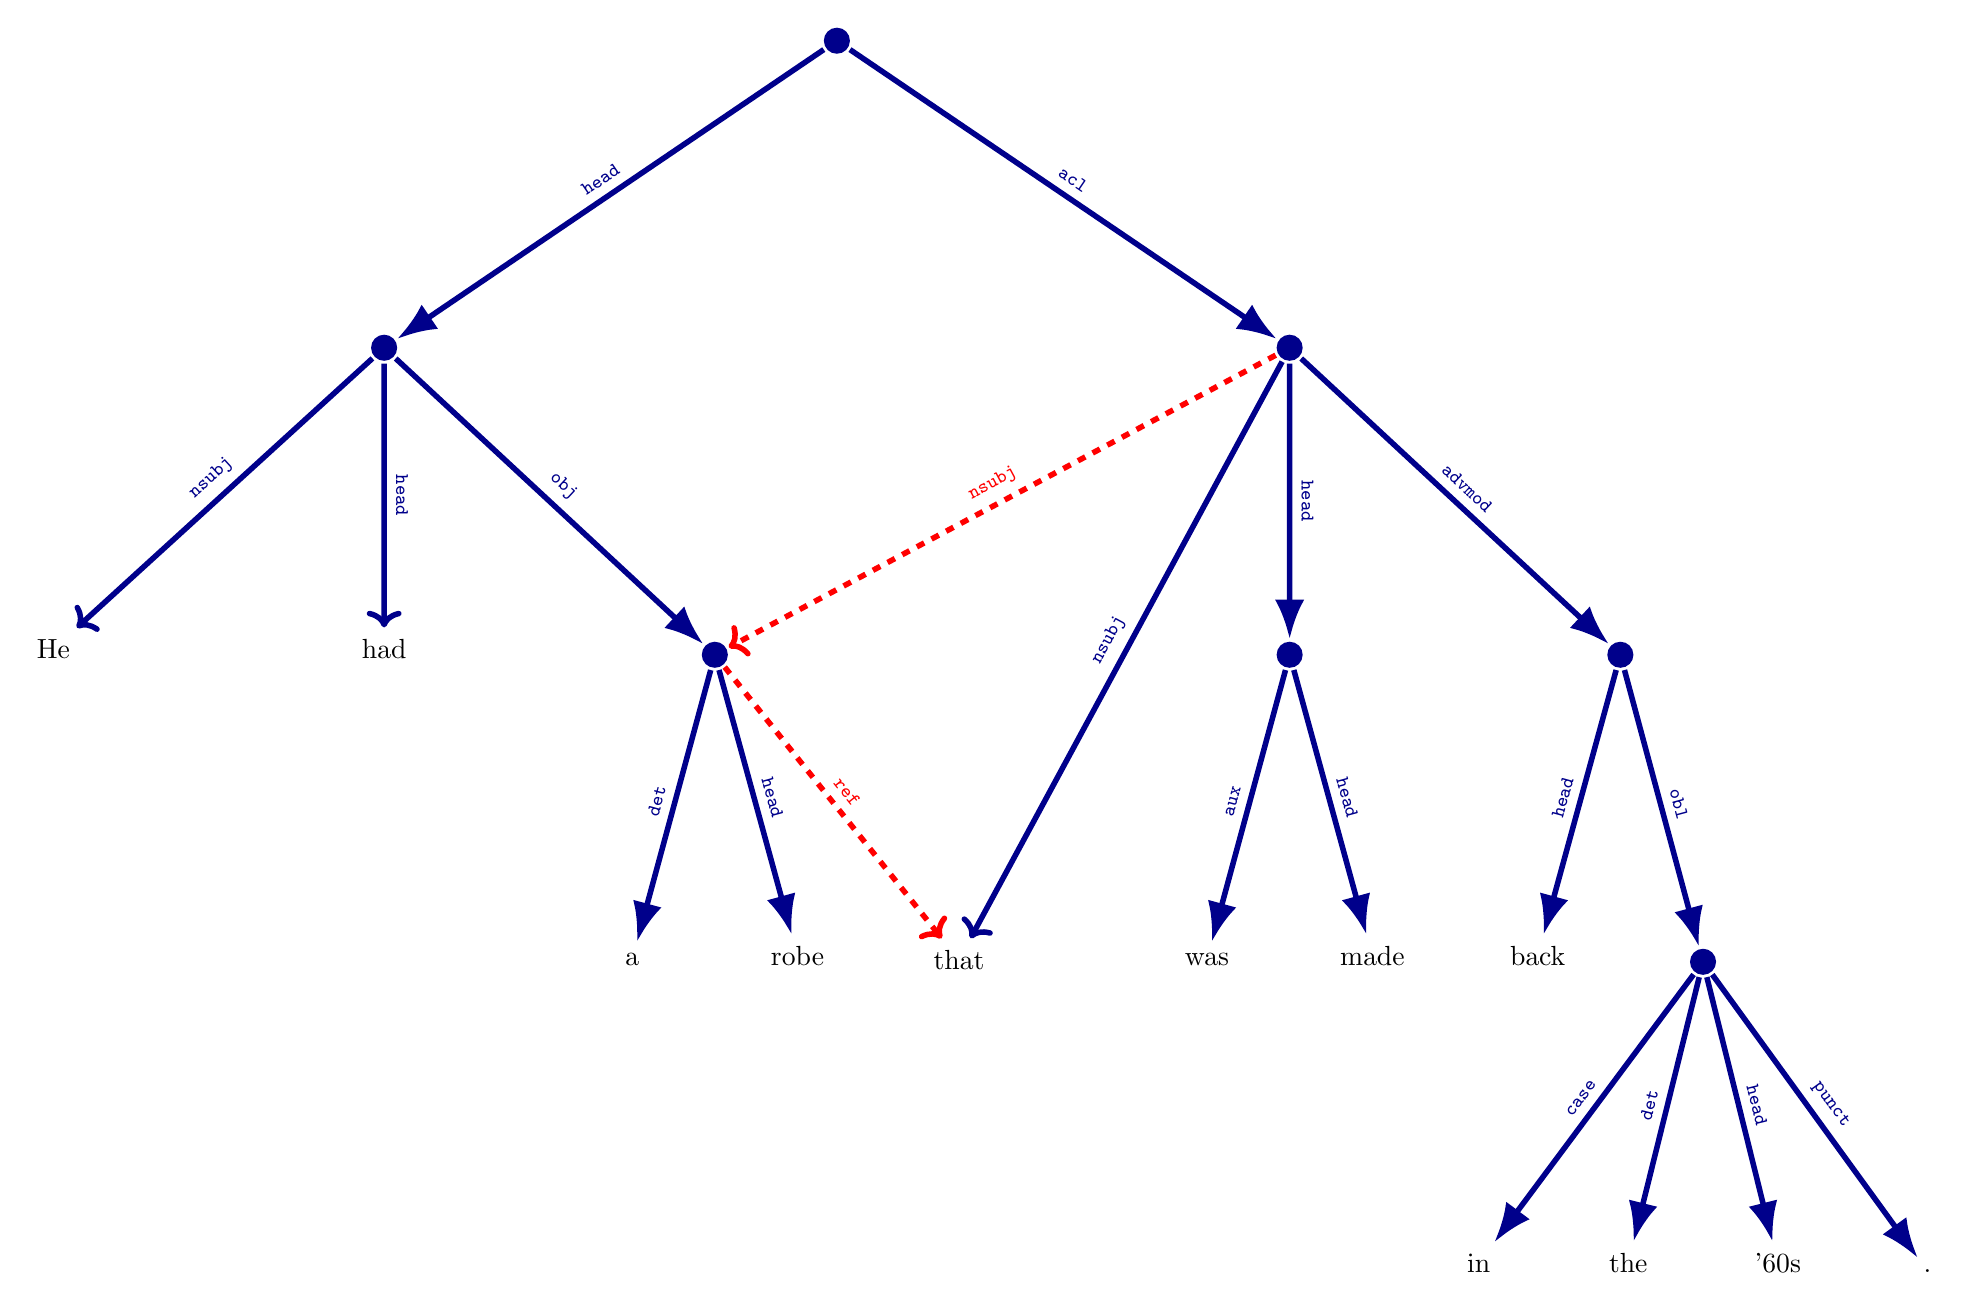
\begin{tikzpicture}[-{Latex[length=5mm]}, color=DarkBlue, line width=2pt,
      every node/.append style={sloped,anchor=south,auto=false,font=\scriptsize\ttfamily},
      level distance=41mm,
	  level 1/.style={sibling distance=115mm},
	  level 2/.style={sibling distance=42mm},
	  level 3/.style={sibling distance=21mm},
	  level 4/.style={sibling distance=19mm},
	  every circle node/.append style={fill=DarkBlue}]
	  \tikzstyle{word} = [font=\rmfamily,color=black]
	  \node (1_1) [circle] {}
	  {
	  child {node (1_2) [circle] {}
	    {
	    child {node (1_6) [word] {He}  edge from parent [draw=none]}
	    child {node (1_3) [word] {had}  edge from parent [draw=none]}
	    child {node (1_7) [circle] {}
	      {
	      child {node (1_14) [word] {a}  edge from parent node[midway,above,sloped]  {\scriptsize det}}
	      child {node (1_8) [word] {robe}  edge from parent node[midway,above,sloped]  {\scriptsize head}}
	      } edge from parent node[midway,above,sloped]  {\scriptsize obj}}
	    } edge from parent node[midway,above,sloped]  {\scriptsize head}}
	  child {node (1_4) [circle] {}
	    {
	    child {node {}
	    {
    	    child {node (1_15) [word] {that}  edge from parent [draw=none]}
    	} edge from parent [draw=none]}
	    child {node (1_5) [circle] {}
	      {
	      child {node (1_9) [word] {was}  edge from parent node[midway,above,sloped]  {\scriptsize aux}}
	      child {node (1_10) [word] {made}  edge from parent node[midway,above,sloped]  {\scriptsize head}}
	      } edge from parent node[midway,above,sloped]  {\scriptsize head}}
	    child {node (1_11) [circle] {}
	      {
	      child {node (1_12) [word] {back}  edge from parent node[midway,above,sloped]  {\scriptsize head}}
	      child {node (1_16) [circle] {}
	        {
	        child {node (1_18) [word] {in}  edge from parent node[midway,above,sloped]  {\scriptsize case}}
	        child {node (1_19) [word] {the}  edge from parent node[midway,above,sloped]  {\scriptsize det}}
	        child {node (1_17) [word] {'60s}  edge from parent node[midway,above,sloped]  {\scriptsize head}}
	        child {node (1_20) [word] {.}  edge from parent node[midway,above,sloped]  {\scriptsize punct}}
	        } edge from parent node[midway,above,sloped]  {\scriptsize obl}}
	      } edge from parent node[midway,above,sloped]  {\scriptsize advmod}}
	    } edge from parent node[midway,above,sloped]  {\scriptsize acl}}
	  };
	  \draw[->] (1_2) to node [midway,above,sloped] {\scriptsize nsubj} (1_6);
	  \draw[->] (1_2) to node [midway,above,sloped] {\scriptsize head} (1_3);
	  \draw[->] (1_4) to node [midway,above,sloped] {\scriptsize nsubj} (1_15);
	  \draw[dashed,red,->] (1_4) to node [midway,above,sloped] {\scriptsize nsubj} (1_7);
	  \draw[dashed,red,->] (1_7) to node [midway,above,sloped] {\scriptsize ref} (1_15);
	\end{tikzpicture}}
\end{minipage}

\begin{tcolorbox}
{\color{Indigo}
\textbf{UCCA} (Universal Conceptual Cognitive Annotation): cross-lingual semantic representation  \cite{abend2013universal}.
Nodes are scenes/concepts.
\textit{Primary edges} form a tree. \textit{Remote edges} (dashed) allow reentrancy.
}

\begin{minipage}{.44\columnwidth}
  \color{Indigo}
  \begin{center}
  \scalebox{.8}{
    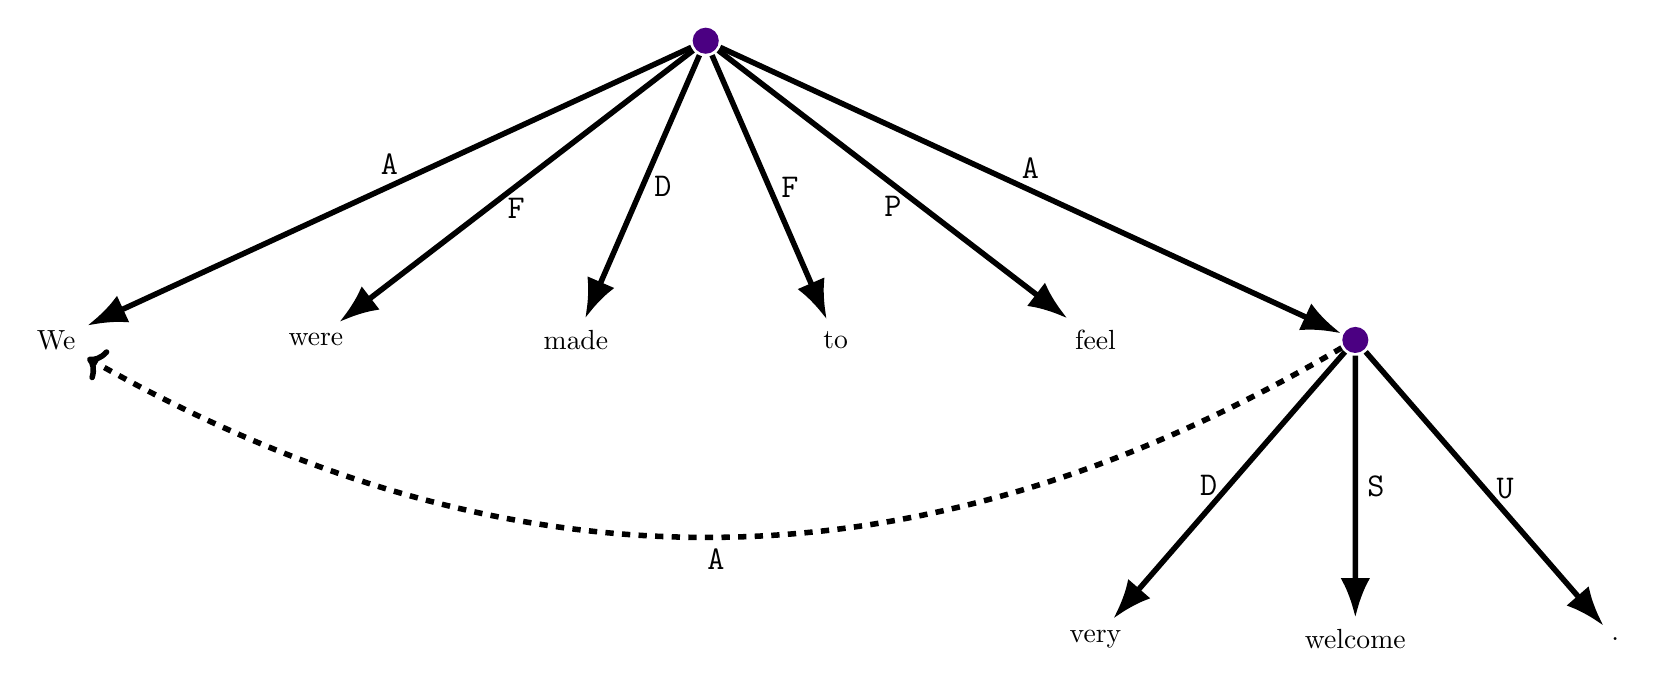
\begin{tikzpicture}[level distance=38mm,sibling distance=33mm, -{Latex[length=5mm]}, line width=2pt,
        every node/.append style={font=\large\ttfamily},
        every circle node/.append style={fill=Indigo}]
      \tikzstyle{word} = [font=\rmfamily,color=black]
      \node (ROOT) [circle] {}
        child {node (We) [word] {We} edge from parent node[above] {A}}
        child {node [word] {were} edge from parent node[below] {F}}
        child {node [word] {made} edge from parent node[right] {D}}
        child {node [word] {to} edge from parent node[right] {F}}
        child {node [word] {feel} edge from parent node[below] {P}}
        child {node (verywelcome) [circle] {}
        {
          child {node [word] {very} edge from parent node[left] {D}}
          child {node [word] {welcome} edge from parent node[right] {S}}
          child {node [word] {.} edge from parent node[right] {U}}
        } edge from parent node[above] {A} }
      ;
      \draw[dashed,->,bend left] (verywelcome) to node [below] {A} (We);
    \end{tikzpicture}
  }
  \end{center}
\end{minipage}
\begin{minipage}{.41\columnwidth}
  \color{Indigo}
  \begin{center}
  \scalebox{.8}{
    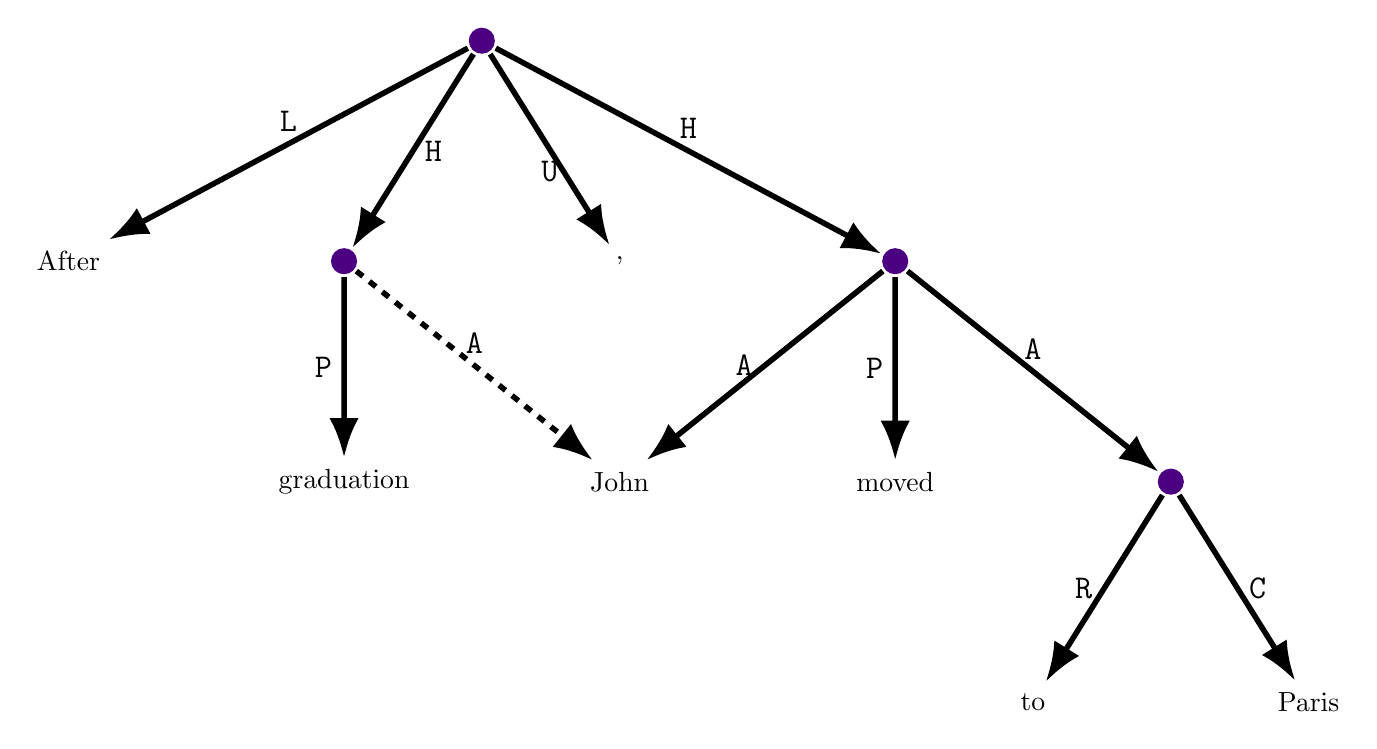
\begin{tikzpicture}[level distance=28mm, sibling distance=35mm, -{Latex[length=5mm]}, line width=2pt,
        every node/.append style={font=\large\ttfamily},
        every circle node/.append style={fill=Indigo}]
      \tikzstyle{word} = [font=\rmfamily,color=black]
      \node (ROOT) [circle] {}
        child {node (After) [word] {After} edge from parent node[above] {L}}
        child {node (graduation) [circle] {}
        {
          child {node [word] {graduation} edge from parent node[left] {P}}
        } edge from parent node[right] {H} }
        child {node [word] {,} edge from parent node[below] {U}}
        child {node (moved) [circle] {}
        {
          child {node (John) [word] {John} edge from parent node[left] {A}}
          child {node [word] {moved} edge from parent node[left] {P}}
          child {node [circle] {}
          {
            child {node [word] {to} edge from parent node[left] {R}}
            child {node [word] {Paris} edge from parent node[right] {C}}
          } edge from parent node[above] {A} }
        } edge from parent node[above] {H} }
        ;
      \draw[dashed,-{Latex[length=5mm]}] (graduation) to node [above] {A} (John);
    \end{tikzpicture}}
  \end{center}
\end{minipage}
\begin{minipage}{.1\columnwidth}
  \begin{center}
  \begin{adjustbox}{margin=2mm,frame,scale=.75,bgcolor=white}
  \color{Indigo}
  \begin{tabular}{>{\ttfamily}cl}
	  P & process \\
	  S & state \\
	  A & participant \\
	  L & linker \\
	  H & linked scene \\
	  C & center \\
	  D & adverbial \\
	  R & relator \\
	  U & punctuation \\
	  F & function \\
  \end{tabular}
  \end{adjustbox}
  \end{center}
\end{minipage}

\end{tcolorbox}


\section*{Enhanced Dependencies}

Some UD treebanks contain enhanced graphs with additional or augmented edges \cite{SCHUSTER16.779,D17-1009}.

\vfill
Conjoined predicates and arguments:

    \begin{dependency}[edge style={-{Latex[length=4mm]}, color=DarkBlue, line width=2pt},
        text only label, label style={above, color=DarkBlue, font=\ttfamily}, font=\small]
    \begin{deptext}[column sep=1em,ampersand replacement=\^]
    he \^ went \^ straight \^ to \^ work \^ and \^ finished \^ the \^ job \^ efficiently \^ and \^ promptly \^ ! \\
    \end{deptext}
        \depedge[edge start x offset=-2pt]{2}{1}{nsubj}
        \depedge[edge below,dashed,red,edge unit distance=.5ex,edge end x offset=2pt]{7}{1}{\color{red}nsubj}
        \deproot[edge unit distance=3ex]{2}{root}
        \depedge[edge start x offset=15pt]{2}{3}{advmod}
        \depedge{5}{4}{mark}
        \depedge[edge unit distance=1.75ex,edge start x offset=10pt]{2}{5}{advcl}
        \depedge[edge start x offset=-3pt]{7}{6}{cc}
        \depedge[edge unit distance=1.5ex,edge start x offset=6pt]{2}{7}{conj}
        \depedge{9}{8}{det}
        \depedge[edge unit distance=2.5ex,edge start x offset=6pt]{7}{9}{obj}
        \depedge[edge unit distance=2.5ex,edge start x offset=2pt]{7}{10}{advmod}
        \depedge{12}{11}{cc}
        \depedge{10}{12}{conj}
        \depedge[edge below,dashed,red,edge unit distance=.65ex,edge end x offset=2pt]{7}{12}{\color{red}advmod}
        \depedge[edge unit distance=1ex,edge start x offset=3pt]{2}{13}{punct}
    \end{dependency}
    
\vfill
Null nodes due to elided predicates, case information:

    \begin{dependency}[edge style={-{Latex[length=4mm]}, color=DarkBlue, line width=2pt},
        text only label, label style={above, color=DarkBlue, font=\ttfamily}, font=\small]
    \begin{deptext}[column sep=1.2em,ampersand replacement=\^]
    I \^ wish \^ all \^ happy \^ holidays \^ , \^ and \^ moreso \^ , \^ \textbf{E9.1} \^ peace \^ on \^ earth \^ . \\
    \end{deptext}
        \depedge[edge start x offset=-2pt]{2}{1}{nsubj}
        \deproot[edge start x offset=-1pt,edge unit distance=4.4ex]{2}{root}
        \depedge[edge start x offset=15pt]{2}{3}{iobj}
        \depedge{5}{4}{amod}
        \depedge[edge start x offset=12pt]{2}{5}{obj}
        \depedge[edge start x offset=-2pt,edge unit distance=2ex]{11}{6}{punct}
        \depedge[edge start x offset=1pt,edge below,dashed,red]{10}{6}{\color{red}punct}
        \depedge[edge start x offset=-3pt,edge unit distance=1.85ex]{11}{7}{cc}
        \depedge[edge start x offset=-6pt,edge below,dashed,red]{10}{7}{\color{red}cc}
        \depedge[edge start x offset=-9pt,edge unit distance=1.5ex]{11}{8}{orphan}
        \depedge[edge start x offset=-6pt,edge below,dashed,red]{10}{8}{\color{red}advmod}
        \depedge[edge start x offset=-12pt,edge unit distance=.8ex]{11}{9}{punct}
        \depedge[edge start x offset=-12pt,edge below,dashed,red]{10}{9}{\color{red}punct}
        \depedge[edge unit distance=1.45ex,edge start x offset=6pt]{2}{11}{conj}
        \depedge[edge below,dashed]{10}{11}{obj}
        \depedge{13}{12}{case}
        \depedge[edge start x offset=1pt]{11}{13}{nmod{\color{red!50}:on}}
        \depedge[edge start x offset=3pt,edge unit distance=1.35ex]{2}{14}{punct}
    \end{dependency}
    
\vfill
\begin{minipage}{.5\columnwidth}
Raising:

    \begin{dependency}[edge style={-{Latex[length=4mm]}, color=DarkBlue, line width=2pt},
        text only label, label style={above, color=DarkBlue, font=\ttfamily}, font=\small]
   \begin{deptext}[column sep=.2em,ampersand replacement=\^]
    We \^ were \^ made \^ to \^ feel \^ very \^ welcome \^ . \\
    \end{deptext}
        \depedge[edge start x offset=1pt]{3}{1}{nsubj:pass}
        \depedge[edge below,dashed,red,edge unit distance=.65ex,edge end x offset=4pt]{5}{1}{\color{red}nsubj:xsubj}
        \depedge[edge below,dashed,red,edge unit distance=.9ex,edge end x offset=-3pt]{7}{1}{\color{red}nsubj:xsubj}
        \depedge[edge start x offset=-3pt]{3}{2}{aux:pass}
        \deproot[edge unit distance=3.4ex]{3}{root}
        \depedge{5}{4}{mark}
        \depedge[edge start x offset=3pt]{3}{5}{xcomp}
        \depedge{7}{6}{advmod}
        \depedge{5}{7}{xcomp}
        \depedge[edge unit distance=2ex,edge start x offset=-1pt]{3}{8}{punct}
    \end{dependency}
\end{minipage}
\begin{minipage}{.5\columnwidth}
Relative clause:

    \begin{dependency}[edge style={-{Latex[length=4mm]}, color=DarkBlue, line width=2pt},
        text only label, label style={above, color=DarkBlue, font=\ttfamily}, font=\small]
    \begin{deptext}[column sep=.1em,ampersand replacement=\^]
    He \^ had \^ a \^ robe \^ that \^ was \^ made \^ back \^ in \^ the \^ '60s \^ . \\
    \end{deptext}
        \depedge[edge start x offset=-3pt]{2}{1}{nsubj}
        \deproot[edge start x offset=-1pt,edge unit distance=3.355ex]{2}{root}
        \depedge[edge start x offset=-3pt]{4}{3}{det}
        \depedge[edge start x offset=6pt]{2}{4}{obj}
        \depedge[edge start x offset=-3pt,edge unit distance=1.5ex,edge below,dashed,red]{7}{4}{\color{red}nsubj:pass}
        \depedge[edge start x offset=-3pt]{7}{5}{nsubj:pass}
        \depedge[edge start x offset=4pt,edge below,dashed,red]{4}{5}{\color{red}ref}
        \depedge[edge start x offset=-9pt,edge unit distance=2ex]{7}{6}{aux:pass}
        \depedge[edge start x offset=3pt,edge unit distance=2.75ex]{4}{7}{acl:relcl}
        \depedge[edge start x offset=3pt]{7}{8}{advmod}
        \depedge{11}{9}{case}
        \depedge[edge start x offset=-3pt]{11}{10}{det}
        \depedge[edge unit distance=1ex,edge below,dashed,red]{8}{11}{\color{red}obl}
        \depedge[edge start x offset=3pt,edge unit distance=1.2ex]{2}{12}{punct}
    \end{dependency}
\end{minipage}

\vfill
\hrule


\section*{Results}

\begin{minipage}{.5\columnwidth}
	\begin{tabular}{lccc}
	&  TUPA &  TUPA &  UDPipe \\
	&  \small(official) &  \small(unofficial) &  \small(baseline) \\
	All treebanks & 53.69 & 58.48 & 65.80 \\
	Big treebanks & 62.07 & 67.36 & 74.14 \\
	PUD treebanks & 56.35 & 56.82 & 66.63 \\
	Small treebanks & 36.74 & 41.19 & 55.01 \\
	Low-resource & 8.53 & 12.68 & 17.17
	\end{tabular}
	\captionsetup{justification=centering}
	\captionof{table}{Macro-averaged \textbf{LAS-F1} on test treebanks.}
    \vspace{5mm}
    \textbf{\color{DarkBlue} TUPA: first general parser for enhanced UD.}
\end{minipage}
\hfill
\begin{minipage}{.45\columnwidth}
	\begin{tabular}{lcc}
	& \multirow{2}{*}{ LAS-F1} &  Enhanced \\
	& &  LAS-F1 \\
	TUPA (unofficial) & 72.10 & 57.13 \\
	$-$NER & 71.82 & 54.65\\ 
	$-$POS & 69.23 & 49.12\\ 
	$-$Embed. & 72.33 & 54.54\\ 
	$-$Remote & 72.08 & 0.00\\ 
	\hline
	UDPipe & 77.62 & 0.00\\
	UDPipe + CoreNLP & 76.66 & 21.68
	\end{tabular}
	\captionsetup{justification=centering}
	\captionof{table}{Ablation + baselines on \textbf{English EWT} dev.}
\end{minipage}



\begin{minipage}{.5\columnwidth}
\color{DarkSlateGray}
\tiny\titleformat*{\section}{\small}
\setlength\bibitemsep{0pt}
\bibliographystyle{plain}
\bibliography{references}
\end{minipage}
\begin{minipage}{.5\columnwidth}
\color{Black}
\begin{adjustbox}{margin=3mm,frame,minipage=1.15\columnwidth}
\centering\Large
Please join the CoNLL 2019 Shared Task: \\
Cross-Framework Meaning Representation Parsing \\
\Large\texttt{{\color{violet}mrp}.{\color{red}nlpl}.{\color{blue}eu}}
\end{adjustbox}
\end{minipage}


\end{document}
